\documentclass[tikz,border=10pt]{standalone}
\usepackage{amsmath}
\usepackage{amssymb}
\usepackage{tikz}
\usetikzlibrary{arrows.meta,calc,decorations.pathreplacing,patterns,shapes.geometric,positioning,shadings,decorations.pathmorphing}

\begin{document}
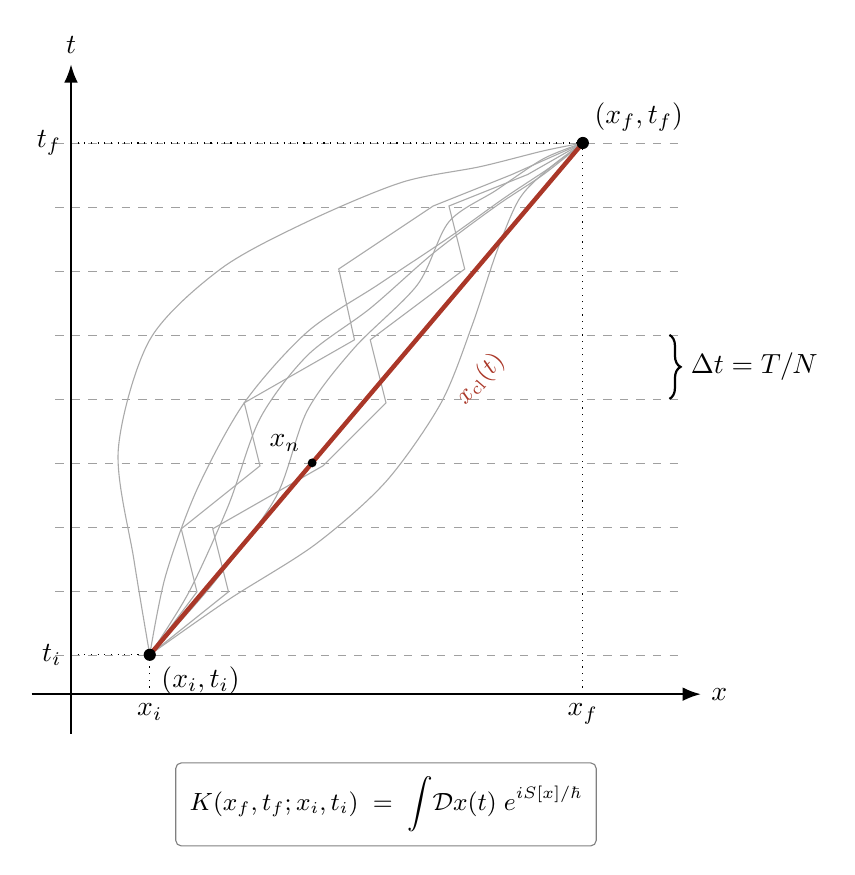
\begin{tikzpicture}[>=Latex,scale=1.0]

% Colors
\definecolor{brickred}{RGB}{170,55,40}
\definecolor{lightgray1}{RGB}{170,170,170}
\definecolor{slicegray}{RGB}{160,160,160}

% Coordinates
\def\xmin{-0.5}
\def\xmax{8.0}
\def\tmin{-0.5}
\def\tmax{8.0}

% Endpoints
\coordinate (A) at (1.0, 0.5);   % (x_i, t_i)
\coordinate (B) at (6.5, 7.0);   % (x_f, t_f)

% Time slices (N = 8)
\foreach \k in {0,1,2,3,4,5,6,7,8} {%
  \pgfmathsetmacro{\ty}{0.5 + \k*0.8125}
  \draw[slicegray, dashed, very thin] (-0.2,\ty) -- (7.8,\ty);
}

% Axes
\draw[->, thick] (\xmin,0) -- (\xmax,0) node[right] {$x$};
\draw[->, thick] (0,\tmin) -- (0,\tmax) node[above] {$t$};

% Time labels at endpoints
\node[left] at (0,0.5) {$t_i$};
\node[left] at (0,7.0) {$t_f$};
\draw[dotted, thin] (0,0.5) -- (1.0,0.5);
\draw[dotted, thin] (0,7.0) -- (6.5,7.0);

% x labels at endpoints
\node[below] at (1.0,0) {$x_i$};
\node[below] at (6.5,0) {$x_f$};
\draw[dotted, thin] (1.0,0) -- (1.0,0.5);
\draw[dotted, thin] (6.5,0) -- (6.5,7.0);

% Delta t bracket between two adjacent slices (between k=4 and k=5)
\draw[decorate, decoration={brace, amplitude=4pt, mirror}, thick]
  (7.6, 3.75) -- (7.6, 4.5625) node[midway, right=4pt] {$\Delta t = T/N$};

% Deviated paths (light gray, thin), all pinned to A and B
% Path 1: gentle wavy
\draw[lightgray1, thin] plot[smooth] coordinates {
  (1.0,0.5) (1.5,1.3) (2.0,2.4) (2.4,3.5) (3.0,4.3)
  (3.8,4.9) (4.6,5.6) (5.4,6.2) (6.0,6.6) (6.5,7.0)
};

% Path 2: bows to the left
\draw[lightgray1, thin] plot[smooth] coordinates {
  (1.0,0.5) (1.2,1.5) (1.6,2.6) (2.2,3.7) (3.0,4.6)
  (3.9,5.2) (4.8,5.8) (5.5,6.3) (6.1,6.7) (6.5,7.0)
};

% Path 3: bows to the right
\draw[lightgray1, thin] plot[smooth] coordinates {
  (1.0,0.5) (2.0,1.2) (3.1,1.9) (4.0,2.7) (4.7,3.7)
  (5.1,4.7) (5.4,5.6) (5.7,6.3) (6.1,6.7) (6.5,7.0)
};

% Path 4: zigzag (jagged)
\draw[lightgray1, thin]
  (1.0,0.5) -- (1.6,1.3) -- (1.4,2.1) -- (2.4,2.9) -- (2.2,3.7)
  -- (3.6,4.5) -- (3.4,5.4) -- (4.6,6.2) -- (5.6,6.6) -- (6.5,7.0);

% Path 5: another zigzag
\draw[lightgray1, thin]
  (1.0,0.5) -- (2.0,1.3) -- (1.8,2.1) -- (3.2,2.9) -- (4.0,3.7)
  -- (3.8,4.5) -- (5.0,5.4) -- (4.8,6.2) -- (5.8,6.6) -- (6.5,7.0);

% Path 6: large left arc
\draw[lightgray1, thin] plot[smooth] coordinates {
  (1.0,0.5) (0.8,1.7) (0.6,3.1) (1.0,4.5) (1.9,5.4)
  (3.0,6.0) (4.2,6.5) (5.2,6.7) (6.0,6.9) (6.5,7.0)
};

% Path 7: undulating
\draw[lightgray1, thin] plot[smooth] coordinates {
  (1.0,0.5) (1.8,1.4) (2.6,2.5) (3.0,3.6) (3.6,4.4)
  (4.4,5.2) (4.8,6.0) (5.4,6.4) (6.0,6.8) (6.5,7.0)
};

% Classical path (brickred, bold) — straight line A to B
\draw[brickred, line width=1.6pt] (A) -- (B);

% Mark a representative slice point x_n on classical path
% At slice k=3: t = 0.5 + 3*0.8125 = 2.9375
% Classical path: x(t) = 1.0 + (6.5-1.0)*(t-0.5)/(7.0-0.5) = 1.0 + 5.5*(t-0.5)/6.5
% At t=2.9375: x = 1.0 + 5.5*2.4375/6.5 = 1.0 + 2.0625 = 3.0625
\fill[black] (3.0625, 2.9375) circle (1.6pt);
\node[above left=1pt, black] at (3.0625, 2.9375) {$x_n$};

% Endpoints (black dots)
\fill[black] (A) circle (2.2pt);
\fill[black] (B) circle (2.2pt);

% Endpoint labels
\node[below right=1pt] at (A) {$(x_i,t_i)$};
\node[above right=1pt] at (B) {$(x_f,t_f)$};

% Label classical path
\node[brickred, font=\small] at (5.2, 4.0) [rotate=49] {$x_{\mathrm{cl}}(t)$};

% Formula box on the right
\node[draw=black!50, fill=white, rounded corners=2pt, inner sep=5pt, font=\small]
  at (4.0, -1.4)
  {$\displaystyle K(x_f,t_f;x_i,t_i)\;=\;\int\!\mathcal D x(t)\;e^{iS[x]/\hbar}$};

\end{tikzpicture}
\end{document}
